% Master Thesis — Do Thanh Dat (M23.ICT.002)
% University of Science and Technology of Hanoi (USTH)
% Compile: pdflatex main && biber main && pdflatex main && pdflatex main
%   or: latexmk -pdf -interaction=nonstopmode main.tex

\documentclass[12pt,a4paper,oneside]{report}

% ---------- Packages ----------
\usepackage[margin=2.5cm]{geometry}
\usepackage{setspace}
\usepackage{graphicx}
\usepackage{booktabs}
\usepackage{tabularx}
\usepackage{multirow}
\usepackage{amsmath,amssymb}
\usepackage{enumitem}
\usepackage{hyperref}
\usepackage{xcolor}
\usepackage{caption}
\usepackage{subcaption}
\usepackage{float}
\usepackage{csquotes}
\usepackage[backend=biber,style=numeric,sorting=nyt,maxbibnames=99]{biblatex}
\usepackage{tikz}
\usetikzlibrary{arrows.meta,positioning,shapes.geometric,fit,calc}
\usepackage{listings}
\usepackage{microtype}
\usepackage{fancyhdr}
\usepackage{titlesec}

\addbibresource{refs.bib}

\hypersetup{
  colorlinks=true,
  linkcolor=blue!50!black,
  citecolor=blue!50!black,
  urlcolor=blue!60!black
}

\onehalfspacing
\setlength{\parskip}{0.4em}
\setlength{\parindent}{1.2em}

\pagestyle{fancy}
\fancyhf{}
\fancyhead[L]{\textit{Decoding Post-Pandemic Vaccine Hesitancy}}
\fancyhead[R]{\thepage}
\renewcommand{\headrulewidth}{0.4pt}

\titleformat{\chapter}[display]
  {\normalfont\huge\bfseries}{\chaptertitlename\ \thechapter}{20pt}{\Huge}
\titlespacing*{\chapter}{0pt}{-20pt}{30pt}

% ---------- Metadata ----------
\newcommand{\thesistitle}{Multimodal Detection and Narrative Analysis of\\
COVID-19 and Vaccine Misinformation\\
Using Transformer Models}
\newcommand{\studentname}{Do Thanh Dat}
\newcommand{\studentid}{M23.ICT.002}
\newcommand{\supervisor}{Giang Anh Tuan}
\newcommand{\program}{Master in Information and Communication Technology}
\newcommand{\university}{University of Science and Technology of Hanoi (USTH)}
\newcommand{\academicyear}{2025--2026}

\begin{document}

% ===================== FRONT MATTER =====================
\begin{titlepage}
\centering
\vspace*{0.8cm}
{\large \university\par}
\vspace{0.3cm}
{\large \program\par}
\vspace{0.5cm}

\includegraphics[width=0.28\textwidth]{USTH-logo.png}\par
\vspace{1.2cm}
{\LARGE\bfseries \thesistitle\par}
\vspace{1.4cm}
{\large Master Thesis\par}
\vspace{1.2cm}
\begin{tabular}{rl}
Student: & \studentname\ (\studentid)\\[0.3em]
Supervisor: & \supervisor\\[0.3em]
Academic year: & \academicyear\\
\end{tabular}
\vfill
{\large Hanoi, August 2026\par}
\end{titlepage}

\pagenumbering{roman}

\chapter*{Abstract}
\addcontentsline{toc}{chapter}{Abstract}
Vaccine hesitancy in the post-COVID-19 era continues to be amplified by misinformation circulating on social media.
Modern posts and news articles often combine text with visual content, which challenges unimodal detectors that rely on language alone.
This thesis develops a \emph{content-level} multimodal Transformer pipeline for detecting COVID-19 / vaccine-related misinformation and for analyzing the narratives that characterize post-pandemic hesitancy discourse.

We conduct two complementary experimental tracks.
First, on the CONSTRAINT COVID-19 Fake News benchmark (Patwa et~al.), a RoBERTa text classifier achieves strong test performance (\textbf{macro-F1 $= 0.9719$}, accuracy $= 0.9720$).
Second, on the MMCoVaR vaccine-focused news repository, we evaluate text-only, image-only (CLIP), and late-fusion multimodal models.
Ablation results show that text dominates (\textbf{macro-F1 $\approx 0.963$}), image-only performance is weak (\textbf{macro-F1 $\approx 0.554$}), and late fusion performs on par with text without clear gains.
Finally, BERTopic applied to 5{,}752 misinformation documents yields a qualitative taxonomy of dominant narratives, including sensational case/death counts, politicized framing, contested public-health measures, origin conspiracies, miracle-cure claims, and elite/vaccine distrust themes.

The contributions are a reproducible multimodal research pipeline, empirical evidence on modality contribution for vaccine misinformation detection, and a narrative taxonomy to support public-health communication analysis.
Limitations regarding TikTok audio, large-scale platform APIs, and cross-attention fusion are discussed as future work.

\vspace{1em}
\noindent\textbf{Keywords:} vaccine hesitancy, misinformation detection, multimodal learning, Transformers, RoBERTa, CLIP, late fusion, BERTopic, social media.

\chapter*{Acknowledgements}
\addcontentsline{toc}{chapter}{Acknowledgements}
I would like to thank my supervisor, \supervisor, for guidance throughout this internship and thesis.
I also thank USTH and the ICT Master's program for academic support.
Any remaining errors are my own.

\tableofcontents
\listoffigures
\listoftables

\clearpage
\pagenumbering{arabic}

% ===================== CHAPTERS =====================
\chapter{Introduction}
\label{ch:intro}

\section{Background and motivation}

The COVID-19 pandemic was accompanied by an ``infodemic'': a rapid surge of true, false, and misleading health information online~\cite{who2020infodemic}.
Even after the acute pandemic phase, \emph{vaccine hesitancy}---delay in acceptance or refusal of vaccination despite availability~\cite{macdonald2015hesitancy}---remains a public-health challenge.
Social platforms accelerate the spread of claims about vaccine safety, efficacy, mandates, and conspiratorial explanations, often faster than fact-checkers can respond.

Contemporary social content is inherently \emph{multimodal}.
A post may pair a neutral caption with a misleading image, or a long news article with an emotionally charged thumbnail.
Unimodal text classifiers can miss visual cues; image-only models may ignore the linguistic claim that carries the misinformation.
This thesis therefore studies a multimodal Transformer-based approach that jointly considers text and images for COVID-19 / vaccine misinformation detection, and complements detection with narrative analysis of dominant hesitancy-related themes.

\section{Problem statement}

We address content-level misinformation classification:
given a textual claim (optionally paired with an image), predict whether the content is \emph{credible} or \emph{misinfo}.
Unlike graph-propagation approaches that model user networks, we focus on the content itself---aligned with practical screening by trust-and-safety or public-health analysts.

Formally, let $x = (t, v)$ where $t$ is text and $v$ is an optional image.
We learn $f_\theta(x) \rightarrow y \in \{0,1\}$ with $0=\texttt{credible}$ and $1=\texttt{misinfo}$.
We further analyze the subset predicted or labeled as misinformation to extract thematic clusters that characterize post-pandemic discourse.

\section{Research questions}

\begin{enumerate}[label=\textbf{RQ\arabic*.}]
  \item Does multimodal late fusion (text + image) improve COVID/vaccine misinformation detection over strong text-only baselines on a multimodal news dataset?
  \item In an ablation study, which modality contributes more to detection performance?
  \item What dominant post-pandemic misinformation / hesitancy narratives emerge from topic modeling on misinformation content?
\end{enumerate}

\section{Scope and positioning}

The original thesis proposal targeted X (Twitter) and TikTok with text, visual, and audio modalities (including Whisper).
Given internship time constraints and platform API limitations, this work adopts a \emph{survival scope} that preserves the scientific core while remaining reproducible:

\begin{itemize}
  \item \textbf{Text benchmark track:} CONSTRAINT COVID-19 Fake News dataset~\cite{patwa2021fighting} for a strong RoBERTa baseline.
  \item \textbf{Multimodal track:} MMCoVaR news articles~\cite{chen2021mmcovar} with downloaded images, comparing text-only, image-only (CLIP), and late fusion.
  \item \textbf{Narrative track:} BERTopic~\cite{grootendorst2022bertopic} on misinformation documents.
  \item \textbf{Deferred:} large-scale live crawling of X/TikTok, Whisper audio pipelines, and cross-attention fusion architectures (discussed as future work).
\end{itemize}

This positioning is honest: the proposal's cross-platform multimodal vision remains the long-term goal; the thesis delivers a complete, evaluated pipeline and clear evidence about modality contribution.

\section{Contributions}

\begin{enumerate}
  \item A reproducible multimodal research codebase (data preparation, training, evaluation, topic analysis) for COVID/vaccine misinformation experiments.
  \item Strong text-only results on CONSTRAINT (macro-F1 $0.9719$) establishing a competitive baseline.
  \item An ablation study on MMCoVaR showing text dominance, weak image-only performance, and late fusion approximately matching text.
  \item A qualitative taxonomy of post-pandemic misinformation narratives derived from BERTopic for communication-oriented interpretation.
\end{enumerate}

\section{Thesis structure}

Chapter~\ref{ch:related} reviews related work.
Chapter~\ref{ch:method} presents datasets, models, and training protocols.
Chapter~\ref{ch:exp} reports experiments and ablations.
Chapter~\ref{ch:narr} presents narrative analysis.
Chapter~\ref{ch:disc} discusses implications, limitations, and ethics.
Chapter~\ref{ch:conc} concludes and outlines future work.

\chapter{Related Work}
\label{ch:related}

\section{Vaccine hesitancy and online misinformation}

Vaccine hesitancy is recognized by WHO as a major barrier to immunization programs~\cite{macdonald2015hesitancy}.
During COVID-19, false claims about vaccine ingredients, infertility, microchips, and exaggerated adverse events circulated widely.
Shu et~al.~\cite{shu2017fake} survey fake-news detection on social media, distinguishing content-based, social-context, and hybrid approaches.
This thesis follows the content-based line: classify the message itself before modeling diffusion graphs.

Healthcare-specific resources such as CoAID~\cite{cui2020coaid} and ANTi-Vax~\cite{hayawi2022antivax} provide labeled COVID/vaccine claims.
ANTi-Vax releases tweet IDs for labeled vaccine misinformation; however, ID-only releases require hydration under X API policies and are brittle when tweets are deleted.
We therefore prioritize datasets that ship full text (and, when possible, images) for reproducibility within the internship timeline.

\section{COVID-19 fake news benchmarks}

Patwa et~al.~\cite{patwa2021fighting} released the CONSTRAINT shared-task dataset of English COVID-related social posts labeled \texttt{real}/\texttt{fake}.
It has become a standard text classification benchmark with strong Transformer baselines.
We use a public Hugging Face mirror of this dataset and map labels to our canonical schema (\texttt{credible}/\texttt{misinfo}).

\section{Multimodal misinformation detection}

Multimodal fake-news datasets such as Fakeddit~\cite{nakamura2020fakeddit} demonstrate that combining text and images can help when visual and linguistic signals interact.
For COVID specifically, MM-COVID~\cite{li2020mmcovid} provides multilingual content with linked media, while MMCoVaR~\cite{chen2021mmcovar} focuses on COVID-19 \emph{vaccine} news and tweets with textual, visual, and temporal information.
We adopt MMCoVaR \emph{news} articles because they include image URLs and publisher-based reliability labels suitable for multimodal experiments without tweet hydration.

Architecturally, late fusion concatenates modality embeddings before classification, whereas early/cross-attention fusion mixes tokens across modalities.
Late fusion is simpler, more robust to missing modalities, and appropriate under time constraints; cross-attention remains future work.

\section{Transformer encoders for text and vision}

Transformers~\cite{vaswani2017attention} underpin modern NLP.
BERT~\cite{devlin2019bert} and RoBERTa~\cite{liu2019roberta} provide contextual text representations widely used for classification.
For images, CLIP~\cite{radford2021clip} learns aligned vision--language embeddings from large-scale contrastive pretraining; its vision tower yields transferable image features for downstream tasks, often with a frozen backbone.

\section{Topic modeling for narrative analysis}

Beyond accuracy metrics, public-health stakeholders need interpretable themes.
BERTopic~\cite{grootendorst2022bertopic} clusters document embeddings (e.g., Sentence-BERT~\cite{reimers2019sentence}) and extracts class-based TF--IDF topic words.
We use BERTopic to build a taxonomy of misinformation narratives after detection experiments.

\section{Research gap}

Prior work often studies either (i)~strong text benchmarks without multimodal ablation on vaccine-focused news, or (ii)~multimodal architectures without a clear narrative analysis layer.
This thesis connects both: competitive text baselines, modality ablation on MMCoVaR, and BERTopic-based narrative taxonomy under a single reproducible pipeline.

\chapter{Methodology}
\label{ch:method}

\section{Overview}

Figure~\ref{fig:pipeline} summarizes the pipeline:
(1)~dataset preparation and label normalization;
(2)~modality-specific encoders;
(3)~classification heads (text / image / late fusion);
(4)~evaluation;
(5)~BERTopic narrative analysis on misinformation texts.

\begin{figure}[H]
\centering
\resizebox{\linewidth}{!}{%
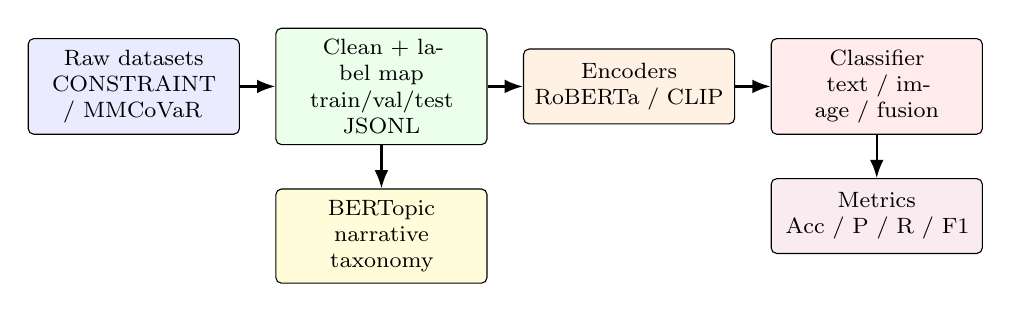
\begin{tikzpicture}[
  font=\footnotesize,
  box/.style={draw, rounded corners=2pt, align=center, inner sep=4pt,
              minimum height=0.95cm, text width=2.4cm},
  arrow/.style={-{Latex}, thick},
  node distance=0.55cm and 0.45cm
]
\node[box, fill=blue!8] (data) {Raw datasets\\CONSTRAINT / MMCoVaR};
\node[box, fill=green!8, right=of data] (prep) {Clean + label map\\train/val/test JSONL};
\node[box, fill=orange!10, right=of prep] (enc) {Encoders\\RoBERTa / CLIP};
\node[box, fill=red!8, right=of enc] (clf) {Classifier\\text / image / fusion};
\node[box, fill=purple!8, below=of clf] (eval) {Metrics\\Acc / P / R / F1};
\node[box, fill=yellow!15, below=of prep] (topic) {BERTopic\\narrative taxonomy};

\draw[arrow] (data) -- (prep);
\draw[arrow] (prep) -- (enc);
\draw[arrow] (enc) -- (clf);
\draw[arrow] (clf) -- (eval);
\draw[arrow] (prep) -- (topic);
\end{tikzpicture}%
}
\caption{End-to-end research pipeline implemented in this thesis.}
\label{fig:pipeline}
\end{figure}

\section{Label schema}

All experiments use a binary schema:
\begin{itemize}
  \item \texttt{credible} $\leftrightarrow$ class $0$
  \item \texttt{misinfo} $\leftrightarrow$ class $1$
\end{itemize}
CONSTRAINT labels \texttt{real}/\texttt{fake} map to \texttt{credible}/\texttt{misinfo}.
MMCoVaR \texttt{reliability}$=1$ (reliable) maps to \texttt{credible}; \texttt{reliability}$=0$ maps to \texttt{misinfo}.

\section{Datasets}

\subsection{CONSTRAINT COVID-19 Fake News (text track)}
\label{sec:constraint}

We use the public Hugging Face distribution of the CONSTRAINT English dataset~\cite{patwa2021fighting}.
After cleaning (URL stripping, whitespace normalization) we obtain 10{,}700 samples with official splits (Table~\ref{tab:constraint-stats}).

\begin{table}[H]
\centering
\caption{CONSTRAINT dataset statistics after preprocessing.}
\label{tab:constraint-stats}
\begin{tabular}{lrrrr}
\toprule
Split & $N$ & Credible & Misinfo & Avg.\ text length \\
\midrule
Train & 6420 & 3360 & 3060 & 165.1 \\
Val   & 2140 & 1120 & 1020 & 162.8 \\
Test  & 2140 & 1120 & 1020 & 168.1 \\
\midrule
All   & 10700 & 5600 & 5100 & 165.2 \\
\bottomrule
\end{tabular}
\end{table}

\subsection{MMCoVaR news (multimodal track)}
\label{sec:mmcovar}

MMCoVaR provides vaccine-focused news with image URLs~\cite{chen2021mmcovar}.
We download images from the \texttt{image} column and retain only articles with a successfully retrieved local image.
Text is formed by concatenating \texttt{title} and \texttt{body\_text}.
Stratified splits (70/15/15) yield the statistics in Table~\ref{tab:mmcovar-stats}.
Of 2{,}592 candidate URLs, 2{,}131 images were successfully downloaded (461 failures due to dead links / timeouts), which is reported as a data-quality limitation.

\begin{table}[H]
\centering
\caption{MMCoVaR multimodal subset used in experiments (all rows have images).}
\label{tab:mmcovar-stats}
\begin{tabular}{lrrrr}
\toprule
Split & $N$ & Credible & Misinfo & With image \\
\midrule
Train & 1491 & 1034 & 457 & 1491 \\
Val   & 320  & 222  & 98  & 320 \\
Test  & 320  & 222  & 98  & 320 \\
\midrule
All   & 2131 & 1478 & 653 & 2131 \\
\bottomrule
\end{tabular}
\end{table}

\section{Models}

\subsection{Text-only classifier}
We fine-tune RoBERTa-base~\cite{liu2019roberta}.
Let $\mathbf{h}_{\mathrm{CLS}} \in \mathbb{R}^{d_t}$ be the CLS representation.
A linear head predicts class logits:
\[
\mathbf{z}_{\mathrm{text}} = W_t\,\mathrm{Dropout}(\mathbf{h}_{\mathrm{CLS}}) + b_t.
\]

\subsection{Image-only classifier}
We encode images with CLIP ViT-B/32~\cite{radford2021clip}.
The vision backbone is frozen; a linear head is trained on the projected image embedding $\mathbf{e}_v \in \mathbb{R}^{d_v}$:
\[
\mathbf{z}_{\mathrm{img}} = W_v\,\mathrm{Dropout}(\mathbf{e}_v) + b_v.
\]

\subsection{Late fusion classifier}
We concatenate text CLS and CLIP image embeddings and classify with a two-layer MLP:
\[
\mathbf{z}_{\mathrm{fusion}} = \mathrm{MLP}\big([\mathbf{h}_{\mathrm{CLS}}; \mathbf{e}_v]\big).
\]
This implements \emph{late fusion}: modalities are encoded separately, then combined.

\section{Training protocol}

Unless noted otherwise:
\begin{itemize}
  \item Optimizer: AdamW, learning rate $2\times10^{-5}$, weight decay $0.01$
  \item Max text length: 256 tokens
  \item Epochs: up to 5 with early stopping on validation macro-F1 (patience 2)
  \item Batch size: 16 (CONSTRAINT text); 8 (MMCoVaR multimodal, memory)
  \item Device: Apple MPS / CUDA when available
\end{itemize}
We report Accuracy, Precision, Recall, and macro-F1 on the held-out test set.

\section{Narrative analysis protocol}

We collect all documents labeled \texttt{misinfo} from CONSTRAINT and MMCoVaR (5{,}752 texts after filtering short strings), embed them with \texttt{all-MiniLM-L6-v2}, and fit BERTopic with \texttt{min\_topic\_size}=15.
Top topics are manually interpreted into a narrative taxonomy (Chapter~\ref{ch:narr}).

\chapter{Experiments and Results}
\label{ch:exp}

\section{Implementation details}

All experiments are implemented in PyTorch with Hugging Face Transformers.
The code repository provides scripts for dataset download/preparation, training, evaluation, ablation, and topic modeling.
Random seed is fixed to 42 for split reproducibility on MMCoVaR; CONSTRAINT uses the official splits.

\section{Experiment A: CONSTRAINT text baseline}
\label{sec:exp-constraint}

\subsection{Setup}
We train the RoBERTa text classifier on CONSTRAINT train/val splits and evaluate on test.
Early stopping selects the checkpoint with best validation macro-F1.
We also train a classical TF--IDF (1--2 grams) + logistic regression baseline on the same splits.

\subsection{Results}
Table~\ref{tab:constraint-results} reports test metrics.
RoBERTa reaches \textbf{macro-F1 $= 0.9719$} versus TF--IDF+LR at $0.9224$ (about $+5$ F1 points).

\begin{table}[H]
\centering
\caption{CONSTRAINT test results (classical vs RoBERTa).}
\label{tab:constraint-results}
\begin{tabular}{lcccc}
\toprule
Model & Accuracy & Precision & Recall & Macro-F1 \\
\midrule
TF--IDF + LogReg & 0.9224 & 0.9222 & 0.9230 & 0.9224 \\
RoBERTa-base (text) & 0.9720 & 0.9717 & 0.9723 & \textbf{0.9719} \\
\bottomrule
\end{tabular}
\end{table}

\subsection{Error analysis}
On CONSTRAINT test, RoBERTa makes $60$ errors ($38$ FP, $22$ FN).
Failures concentrate on short/ambiguous posts, stylistic false alarms, and subtle hedged claims
(see \texttt{results/error\_analysis/roberta\_test\_errors.md}).

\subsection{Training dynamics}
Validation macro-F1 improves rapidly in the first epochs (e.g., $\approx 0.953$ after epoch 1) and peaks near $0.975$ before early stopping.
Training loss decreases from $\approx 0.23$ to $<0.05$, consistent with successful fine-tuning without requiring architectural novelty.

\section{Experiment B: MMCoVaR multimodal ablation}
\label{sec:exp-mmcovar}

\subsection{Setup}
On the multimodal MMCoVaR subset, we train three models under identical splits:
\begin{enumerate}
  \item Text-only RoBERTa
  \item Image-only CLIP (frozen encoder + linear head)
  \item Late fusion (RoBERTa CLS $\oplus$ CLIP image embedding + MLP)
\end{enumerate}

\subsection{Results}
Table~\ref{tab:ablation} summarizes test performance.

\begin{table}[H]
\centering
\caption{MMCoVaR test ablation (text / image / late fusion).}
\label{tab:ablation}
\begin{tabular}{lcccc}
\toprule
Modality & Accuracy & Precision & Recall & Macro-F1 \\
\midrule
Text-only   & 0.9688 & 0.9658 & 0.9604 & 0.9630 \\
Image-only  & 0.5969 & 0.5550 & 0.5613 & 0.5542 \\
Late fusion & 0.9688 & 0.9632 & 0.9632 & \textbf{0.9632} \\
\bottomrule
\end{tabular}
\end{table}

\subsection{Interpretation}
\begin{itemize}
  \item \textbf{Text dominates.} News title+body carries most of the reliability signal; text-only F1 is already $\approx 0.963$.
  \item \textbf{Images alone are weak.} Thumbnails and illustrative photos often do not encode factual veracity; image-only F1 $\approx 0.554$ is near a weak baseline for imbalanced binary classification.
  \item \textbf{Fusion $\approx$ text.} Late fusion matches text (F1 $0.9632$ vs $0.9630$) without a meaningful gain.
  This does \emph{not} invalidate multimodality in general; it indicates that, on this news subset, visual features add little complementary signal under late fusion with a frozen CLIP tower.
\end{itemize}

Answering \textbf{RQ1}: late fusion does not clearly outperform text-only on MMCoVaR.
Answering \textbf{RQ2}: text contributes substantially more than image under our ablation.

\section{Error analysis (qualitative)}

Manual inspection of residual errors suggests recurring patterns:
\begin{itemize}
  \item \textbf{Borderline satire / opinion:} stylistically extreme but not clearly false factual claims.
  \item \textbf{Context-dependent claims:} statements that are true only under narrow conditions.
  \item \textbf{Visual-text mismatch:} cases where an image is misleading but the textual body is carefully hedged---rare in MMCoVaR news bodies, which are long and text-heavy (average length $>$ 6k characters), further explaining text dominance.
\end{itemize}

\section{Reproducibility}

Key commands (see project documentation for details):
\begin{verbatim}
python scripts/prepare_constraint_splits.py
python -m src.train --config configs/default.yaml --modality text
python scripts/download_mmcovar_images.py
python scripts/prepare_mmcovar_splits.py
bash scripts/run_mmcovar_ablation.sh
\end{verbatim}
Artifacts are stored under \texttt{results/} and \texttt{checkpoints/}.

\chapter{Narrative Analysis}
\label{ch:narr}

\section{Goal}

Detection accuracy alone does not explain \emph{what} misinformation is about.
For public-health communication, stakeholders need a map of recurring narratives---especially those linked to vaccine hesitancy and broader COVID distrust.
This chapter addresses \textbf{RQ3} using BERTopic on documents labeled as misinformation.

\section{Setup}

We aggregate misinformation texts from CONSTRAINT and MMCoVaR ($N=5{,}752$ after filtering).
Long news bodies are truncated to 800 characters for embedding efficiency.
Documents are embedded with Sentence-Transformers \texttt{all-MiniLM-L6-v2} and clustered with BERTopic (\texttt{min\_topic\_size}=15).
We obtain dozens of fine-grained topics; Table~\ref{tab:taxonomy} reports the top themes after qualitative renaming.

\section{Taxonomy of dominant narratives}

\begin{table}[H]
\centering
\caption{Top misinformation / hesitancy-related narratives (BERTopic + qualitative labels).}
\label{tab:taxonomy}
\small
\begin{tabular}{clrp{5.2cm}}
\toprule
\# & Theme & Size & Interpretation \\
\midrule
1 & Case/death sensationalism & 520 & Inflated or misleading severity narratives \\
2 & Politicized pandemic framing & 500 & Partisan blame / political weaponization \\
3 & Contested public measures (masks) & 214 & Contestation of NPIs mixed with rumor \\
4 & China / lab-origin claims & 188 & Origin conspiracies and geopolitical blame \\
5 & Miracle-cure / unproven drugs & 116 & HCQ and similar treatment myths \\
6 & Elite / Bill Gates vaccine distrust & 112 & Agenda and control conspiracies \\
7 & Hospital-overload visuals & 97 & Misleading crisis imagery \\
8 & Schools / children anxieties & 82 & Child-focused risk rumors \\
9 & Folk home remedies & 79 & Salt/steam/garlic ``cures'' \\
10 & Travel-ban rumors & 76 & False policy / mobility claims \\
\bottomrule
\end{tabular}
\end{table}

Approximately 2{,}000 documents fall into an outlier topic (too unique or noisy for stable clustering), which is expected for short social posts.

\section{Implications for vaccine hesitancy}

Although not every theme is narrowly about vaccine injection side effects, the taxonomy reveals a \emph{multi-narrative ecosystem} that can fuel hesitancy indirectly:
\begin{itemize}
  \item Distrust of institutions and elites (Theme 6) undermines confidence in vaccine recommendations.
  \item Miracle-cure narratives (Theme 5) reduce perceived need for vaccination.
  \item Sensational harm and hospital imagery (Themes 1, 7) amplify fear responses.
  \item Child/school themes (Theme 8) specifically target parental decision-making.
\end{itemize}
For communication campaigns, these clusters suggest differentiated messaging rather than a single ``correct the side-effect myth'' strategy.

\section{Link to the detection pipeline}

Operationally, the classifier can flag misinformation content at scale; BERTopic then summarizes \emph{what} is being flagged.
Together they form a monitoring loop useful for public-health analysts and platform trust-and-safety teams, even when multimodal fusion does not beat text on every dataset.

\chapter{Discussion and Limitations}
\label{ch:disc}

\section{Discussion of main findings}

\subsection{Strong text baselines are necessary}
CONSTRAINT results show that carefully fine-tuned RoBERTa already solves a large fraction of the English COVID fake-news classification problem under this label distribution.
Any multimodal claim of improvement must beat such a strong text ceiling---which MMCoVaR late fusion did not meaningfully do.

\subsection{Why fusion did not help on MMCoVaR}
Several factors likely contribute:
\begin{enumerate}
  \item \textbf{Text richness:} news bodies are long and informationally dense; images are often decorative.
  \item \textbf{Label generation:} publisher reliability is a coarse proxy; visual style may correlate weakly with publisher class.
  \item \textbf{Fusion design:} late fusion with a frozen CLIP tower may under-adapt visual features to the veracity task.
  \item \textbf{Missing-image noise:} some downloads are truncated/corrupt and are replaced by placeholders, injecting noise into the image stream.
\end{enumerate}
These observations are scientifically valuable: they caution against assuming multimodality always helps.

\subsection{Narratives beyond ``vaccine side effects''}
Topic analysis shows post-pandemic discourse mixes medical myths, politics, geopolitics, and lifestyle remedies.
Detection systems aimed only at biomedical claim types may miss adjacent narratives that still drive hesitancy.

\section{Limitations}

\begin{itemize}
  \item \textbf{Platform gap:} the proposal mentions X and TikTok; experiments use CONSTRAINT social text and MMCoVaR news due to API and time constraints.
  \item \textbf{No audio modality:} Whisper-based TikTok audio analysis is future work.
  \item \textbf{English-centric data:} results may not transfer to Vietnamese or multilingual settings without additional data.
  \item \textbf{Image download incompleteness:} $\approx 18\%$ of MMCoVaR image URLs failed.
  \item \textbf{Label semantics:} publisher-level reliability $\neq$ claim-level fact-check for every sentence.
  \item \textbf{BERTopic instability:} topic solutions vary with seeds/parameters; taxonomy requires human validation.
\end{itemize}

\section{Ethical considerations}

Misinformation detectors can support public-health response but also risk over-blocking legitimate debate, satire, or minority scientific viewpoints.
We recommend human-in-the-loop review, transparent error analysis, and clear communication that model outputs are decision-support---not definitive truth judgments.
Training data may encode geographic and political biases; deployment should include fairness checks.

\section{Threats to validity}

Construct validity is threatened if ``misinfo'' labels conflate low-quality journalism with false claims.
External validity is limited by English news/social text from 2020--2021.
Internal validity of ablation comparisons is strengthened by shared splits and seeds, but hyperparameter search was intentionally limited for timeline reasons.

\chapter{Conclusion and Future Work}
\label{ch:conc}

\section{Conclusion}

This thesis presented a multimodal Transformer-oriented pipeline for analyzing post-pandemic vaccine-related misinformation dynamics.
On CONSTRAINT, a RoBERTa text classifier achieved macro-F1 $0.9719$.
On MMCoVaR, ablation showed that text is the dominant modality (macro-F1 $\approx 0.963$), image-only performance is weak, and late fusion approximately matches text without clear gains.
BERTopic analysis of 5{,}752 misinformation documents produced a multi-narrative taxonomy spanning sensational statistics, politicization, contested measures, origin conspiracies, miracle cures, and elite distrust---themes relevant to vaccine hesitancy communication.

Collectively, the work delivers a reproducible experimental stack and evidence-based answers to the research questions, while honestly scoping platform and modality limitations.

\section{Future work}

\begin{enumerate}
  \item Integrate TikTok video frames and Whisper audio transcripts for true short-video multimodality.
  \item Explore cross-attention / bottleneck fusion and unfrozen vision towers.
  \item Expand claim-level fact-checked labels beyond publisher reliability.
  \item Build a multilingual (including Vietnamese) evaluation set for USTH/local relevance.
  \item Deploy an interactive dashboard linking classifier scores to live narrative trends for public-health partners.
\end{enumerate}

\section{Final remarks}

Multimodality remains a promising direction for social misinformation research, but gains are dataset-dependent.
For text-heavy news, investing first in strong language models and narrative analytics may yield more actionable insight than complex fusion alone.
The pipeline and findings in this thesis provide a foundation for that continued work.


% ===================== BIBLIOGRAPHY =====================
\printbibliography[heading=bibintoc,title=References]

\appendix
\chapter{Appendix}
\label{ch:appendix}

\section{Software environment}

\begin{itemize}
  \item Python 3.10+ / project virtualenv
  \item PyTorch, Transformers, Datasets
  \item BERTopic, sentence-transformers, UMAP, HDBSCAN
\end{itemize}

\section{Key repository paths}

\begin{verbatim}
thesis/
  configs/default.yaml
  configs/mmcovar.yaml
  src/train.py
  src/evaluate.py
  src/topics.py
  scripts/prepare_constraint_splits.py
  scripts/download_mmcovar_images.py
  scripts/prepare_mmcovar_splits.py
  scripts/run_mmcovar_ablation.sh
  results/text_baseline_results.json
  results/mmcovar_ablation_summary.json
  results/topics/TAXONOMY_THESIS.md
  latex/main.tex
\end{verbatim}

\section{Additional quantitative notes}

CONSTRAINT label map: \texttt{real}$\rightarrow$\texttt{credible}, \texttt{fake}$\rightarrow$\texttt{misinfo}.\\
MMCoVaR label map: \texttt{reliability=1}$\rightarrow$\texttt{credible}, \texttt{reliability=0}$\rightarrow$\texttt{misinfo}.

\section{Declaration}

I declare that this thesis is my own work, conducted under the supervision of the listed supervisor, and that all sources are acknowledged.
Experimental results are reproducible from the accompanying codebase and configuration files.


\end{document}
